% Options for packages loaded elsewhere
\PassOptionsToPackage{unicode}{hyperref}
\PassOptionsToPackage{hyphens}{url}
\PassOptionsToPackage{dvipsnames,svgnames,x11names}{xcolor}
%
\documentclass[
  letterpaper,
  DIV=11,
  numbers=noendperiod]{scrreprt}

\usepackage{amsmath,amssymb}
\usepackage{iftex}
\ifPDFTeX
  \usepackage[T1]{fontenc}
  \usepackage[utf8]{inputenc}
  \usepackage{textcomp} % provide euro and other symbols
\else % if luatex or xetex
  \usepackage{unicode-math}
  \defaultfontfeatures{Scale=MatchLowercase}
  \defaultfontfeatures[\rmfamily]{Ligatures=TeX,Scale=1}
\fi
\usepackage{lmodern}
\ifPDFTeX\else  
    % xetex/luatex font selection
\fi
% Use upquote if available, for straight quotes in verbatim environments
\IfFileExists{upquote.sty}{\usepackage{upquote}}{}
\IfFileExists{microtype.sty}{% use microtype if available
  \usepackage[]{microtype}
  \UseMicrotypeSet[protrusion]{basicmath} % disable protrusion for tt fonts
}{}
\makeatletter
\@ifundefined{KOMAClassName}{% if non-KOMA class
  \IfFileExists{parskip.sty}{%
    \usepackage{parskip}
  }{% else
    \setlength{\parindent}{0pt}
    \setlength{\parskip}{6pt plus 2pt minus 1pt}}
}{% if KOMA class
  \KOMAoptions{parskip=half}}
\makeatother
\usepackage{xcolor}
\setlength{\emergencystretch}{3em} % prevent overfull lines
\setcounter{secnumdepth}{5}
% Make \paragraph and \subparagraph free-standing
\makeatletter
\ifx\paragraph\undefined\else
  \let\oldparagraph\paragraph
  \renewcommand{\paragraph}{
    \@ifstar
      \xxxParagraphStar
      \xxxParagraphNoStar
  }
  \newcommand{\xxxParagraphStar}[1]{\oldparagraph*{#1}\mbox{}}
  \newcommand{\xxxParagraphNoStar}[1]{\oldparagraph{#1}\mbox{}}
\fi
\ifx\subparagraph\undefined\else
  \let\oldsubparagraph\subparagraph
  \renewcommand{\subparagraph}{
    \@ifstar
      \xxxSubParagraphStar
      \xxxSubParagraphNoStar
  }
  \newcommand{\xxxSubParagraphStar}[1]{\oldsubparagraph*{#1}\mbox{}}
  \newcommand{\xxxSubParagraphNoStar}[1]{\oldsubparagraph{#1}\mbox{}}
\fi
\makeatother

\usepackage{color}
\usepackage{fancyvrb}
\newcommand{\VerbBar}{|}
\newcommand{\VERB}{\Verb[commandchars=\\\{\}]}
\DefineVerbatimEnvironment{Highlighting}{Verbatim}{commandchars=\\\{\}}
% Add ',fontsize=\small' for more characters per line
\usepackage{framed}
\definecolor{shadecolor}{RGB}{241,243,245}
\newenvironment{Shaded}{\begin{snugshade}}{\end{snugshade}}
\newcommand{\AlertTok}[1]{\textcolor[rgb]{0.68,0.00,0.00}{#1}}
\newcommand{\AnnotationTok}[1]{\textcolor[rgb]{0.37,0.37,0.37}{#1}}
\newcommand{\AttributeTok}[1]{\textcolor[rgb]{0.40,0.45,0.13}{#1}}
\newcommand{\BaseNTok}[1]{\textcolor[rgb]{0.68,0.00,0.00}{#1}}
\newcommand{\BuiltInTok}[1]{\textcolor[rgb]{0.00,0.23,0.31}{#1}}
\newcommand{\CharTok}[1]{\textcolor[rgb]{0.13,0.47,0.30}{#1}}
\newcommand{\CommentTok}[1]{\textcolor[rgb]{0.37,0.37,0.37}{#1}}
\newcommand{\CommentVarTok}[1]{\textcolor[rgb]{0.37,0.37,0.37}{\textit{#1}}}
\newcommand{\ConstantTok}[1]{\textcolor[rgb]{0.56,0.35,0.01}{#1}}
\newcommand{\ControlFlowTok}[1]{\textcolor[rgb]{0.00,0.23,0.31}{\textbf{#1}}}
\newcommand{\DataTypeTok}[1]{\textcolor[rgb]{0.68,0.00,0.00}{#1}}
\newcommand{\DecValTok}[1]{\textcolor[rgb]{0.68,0.00,0.00}{#1}}
\newcommand{\DocumentationTok}[1]{\textcolor[rgb]{0.37,0.37,0.37}{\textit{#1}}}
\newcommand{\ErrorTok}[1]{\textcolor[rgb]{0.68,0.00,0.00}{#1}}
\newcommand{\ExtensionTok}[1]{\textcolor[rgb]{0.00,0.23,0.31}{#1}}
\newcommand{\FloatTok}[1]{\textcolor[rgb]{0.68,0.00,0.00}{#1}}
\newcommand{\FunctionTok}[1]{\textcolor[rgb]{0.28,0.35,0.67}{#1}}
\newcommand{\ImportTok}[1]{\textcolor[rgb]{0.00,0.46,0.62}{#1}}
\newcommand{\InformationTok}[1]{\textcolor[rgb]{0.37,0.37,0.37}{#1}}
\newcommand{\KeywordTok}[1]{\textcolor[rgb]{0.00,0.23,0.31}{\textbf{#1}}}
\newcommand{\NormalTok}[1]{\textcolor[rgb]{0.00,0.23,0.31}{#1}}
\newcommand{\OperatorTok}[1]{\textcolor[rgb]{0.37,0.37,0.37}{#1}}
\newcommand{\OtherTok}[1]{\textcolor[rgb]{0.00,0.23,0.31}{#1}}
\newcommand{\PreprocessorTok}[1]{\textcolor[rgb]{0.68,0.00,0.00}{#1}}
\newcommand{\RegionMarkerTok}[1]{\textcolor[rgb]{0.00,0.23,0.31}{#1}}
\newcommand{\SpecialCharTok}[1]{\textcolor[rgb]{0.37,0.37,0.37}{#1}}
\newcommand{\SpecialStringTok}[1]{\textcolor[rgb]{0.13,0.47,0.30}{#1}}
\newcommand{\StringTok}[1]{\textcolor[rgb]{0.13,0.47,0.30}{#1}}
\newcommand{\VariableTok}[1]{\textcolor[rgb]{0.07,0.07,0.07}{#1}}
\newcommand{\VerbatimStringTok}[1]{\textcolor[rgb]{0.13,0.47,0.30}{#1}}
\newcommand{\WarningTok}[1]{\textcolor[rgb]{0.37,0.37,0.37}{\textit{#1}}}

\providecommand{\tightlist}{%
  \setlength{\itemsep}{0pt}\setlength{\parskip}{0pt}}\usepackage{longtable,booktabs,array}
\usepackage{calc} % for calculating minipage widths
% Correct order of tables after \paragraph or \subparagraph
\usepackage{etoolbox}
\makeatletter
\patchcmd\longtable{\par}{\if@noskipsec\mbox{}\fi\par}{}{}
\makeatother
% Allow footnotes in longtable head/foot
\IfFileExists{footnotehyper.sty}{\usepackage{footnotehyper}}{\usepackage{footnote}}
\makesavenoteenv{longtable}
\usepackage{graphicx}
\makeatletter
\newsavebox\pandoc@box
\newcommand*\pandocbounded[1]{% scales image to fit in text height/width
  \sbox\pandoc@box{#1}%
  \Gscale@div\@tempa{\textheight}{\dimexpr\ht\pandoc@box+\dp\pandoc@box\relax}%
  \Gscale@div\@tempb{\linewidth}{\wd\pandoc@box}%
  \ifdim\@tempb\p@<\@tempa\p@\let\@tempa\@tempb\fi% select the smaller of both
  \ifdim\@tempa\p@<\p@\scalebox{\@tempa}{\usebox\pandoc@box}%
  \else\usebox{\pandoc@box}%
  \fi%
}
% Set default figure placement to htbp
\def\fps@figure{htbp}
\makeatother

\KOMAoption{captions}{tableheading}
\makeatletter
\@ifpackageloaded{bookmark}{}{\usepackage{bookmark}}
\makeatother
\makeatletter
\@ifpackageloaded{caption}{}{\usepackage{caption}}
\AtBeginDocument{%
\ifdefined\contentsname
  \renewcommand*\contentsname{Table of contents}
\else
  \newcommand\contentsname{Table of contents}
\fi
\ifdefined\listfigurename
  \renewcommand*\listfigurename{List of Figures}
\else
  \newcommand\listfigurename{List of Figures}
\fi
\ifdefined\listtablename
  \renewcommand*\listtablename{List of Tables}
\else
  \newcommand\listtablename{List of Tables}
\fi
\ifdefined\figurename
  \renewcommand*\figurename{Figure}
\else
  \newcommand\figurename{Figure}
\fi
\ifdefined\tablename
  \renewcommand*\tablename{Table}
\else
  \newcommand\tablename{Table}
\fi
}
\@ifpackageloaded{float}{}{\usepackage{float}}
\floatstyle{ruled}
\@ifundefined{c@chapter}{\newfloat{codelisting}{h}{lop}}{\newfloat{codelisting}{h}{lop}[chapter]}
\floatname{codelisting}{Listing}
\newcommand*\listoflistings{\listof{codelisting}{List of Listings}}
\makeatother
\makeatletter
\makeatother
\makeatletter
\@ifpackageloaded{caption}{}{\usepackage{caption}}
\@ifpackageloaded{subcaption}{}{\usepackage{subcaption}}
\makeatother

\usepackage{bookmark}

\IfFileExists{xurl.sty}{\usepackage{xurl}}{} % add URL line breaks if available
\urlstyle{same} % disable monospaced font for URLs
\hypersetup{
  pdftitle={Multilevel Workshop},
  pdfauthor={Andrew Grogan-Kaylor},
  colorlinks=true,
  linkcolor={blue},
  filecolor={Maroon},
  citecolor={Blue},
  urlcolor={Blue},
  pdfcreator={LaTeX via pandoc}}


\title{Multilevel Workshop}
\author{Andrew Grogan-Kaylor}
\date{2025-06-30}

\begin{document}
\maketitle

\renewcommand*\contentsname{Table of contents}
{
\hypersetup{linkcolor=}
\setcounter{tocdepth}{2}
\tableofcontents
}
\listoffigures
\listoftables

\bookmarksetup{startatroot}

\chapter{Introduction}\label{introduction}

This site contains materials for a workshop on multilevel modeling.

\section{Background}\label{background}

Multilevel models are useful when you have data that are nested or
clustered inside social units such as schools, neighborhoods, states, or
countries.

Multilevel models are also useful when you have longitudinal data where
repeated measures are collected for study participants.

\section{Simulated Multilevel Data}\label{simulated-multilevel-data}

The data used in these workshop materials are \emph{simulated} data on
parents, children and families. The data are simulated to come from 30
hypothetical countries around the world. These are the same data used
and discussed in my book
\emph{\href{https://academic.oup.com/book/60530}{Multilevel Thinking:
Discovering Variation, Universals, and Particulars in Cross-Cultural
Research}}.

There are two versions of the data: a \emph{cross-sectional} data set
from a single point in time; a \emph{longitudinal} version of the data
spanning several time points.

\begin{figure}

\centering{

\begin{longtable*}[]{@{}
  >{\centering\arraybackslash}p{(\linewidth - 4\tabcolsep) * \real{0.0833}}
  >{\centering\arraybackslash}p{(\linewidth - 4\tabcolsep) * \real{0.3056}}
  >{\centering\arraybackslash}p{(\linewidth - 4\tabcolsep) * \real{0.4306}}@{}}
\toprule\noalign{}
\begin{minipage}[b]{\linewidth}\centering
pos
\end{minipage} & \begin{minipage}[b]{\linewidth}\centering
variable
\end{minipage} & \begin{minipage}[b]{\linewidth}\centering
label
\end{minipage} \\
\midrule\noalign{}
\endhead
\bottomrule\noalign{}
\endlastfoot
1 & country & country id \\
2 & HDI & Human Development Index \\
3 & family & family id \\
4 & id & unique country family id \\
5 & identity & hypothetical identity group variable \\
6 & intervention & recieved intervention \\
7 & physical\_punishment & physical punishment in past week \\
8 & warmth & parental warmth in past week \\
9 & outcome & beneficial outcome \\
\end{longtable*}

}

\caption{\label{fig-describe}Simulated Multilevel Data}

\end{figure}%

\bookmarksetup{startatroot}

\chapter{Two Level Cross Sectional; And Three Level Longitudinal
Models}\label{two-level-cross-sectional-and-three-level-longitudinal-models}

\section{Cross Sectional Model}\label{cross-sectional-model}

\subsection{Get Data}\label{get-data}

\begin{Shaded}
\begin{Highlighting}[]

\KeywordTok{use} \StringTok{"simulated\_multilevel\_data.dta"}\NormalTok{, }\KeywordTok{clear}
\end{Highlighting}
\end{Shaded}

\subsection{The Equation}\label{the-equation}

\[\text{outcome}_{ij} = \beta_0 + \beta_1 \text{parental warmth} + \beta_2 \text{physical punishment} + \beta_3 \text{time} + \]

\[\beta_4 \text{identity}_2 + \beta_5 \text{intervention} + \beta_6 HDI +\]

\[u_{0j} + u_{1j} \times \text{parental warmth} + e_{ij} \]

\subsection{Descriptive Statistics}\label{descriptive-statistics}

\begin{Shaded}
\begin{Highlighting}[]

\KeywordTok{summarize} \CommentTok{// descriptive statistics}
\end{Highlighting}
\end{Shaded}

\begin{verbatim}
    Variable |        Obs        Mean    Std. dev.       Min        Max
-------------+---------------------------------------------------------
     country |      3,000        15.5    8.656884          1         30
         HDI |      3,000    64.76667    17.24562         33         87
      family |      3,000        50.5    28.87088          1        100
          id |          0
    identity |      3,000    .4976667    .5000779          0          1
-------------+---------------------------------------------------------
intervention |      3,000    .4843333    .4998378          0          1
physical_p~t |      3,000    2.478667    1.360942          0          5
      warmth |      3,000    3.521667    1.888399          0          7
     outcome |      3,000    52.43327    6.530996   29.60798   74.83553
\end{verbatim}

\subsection{Spaghetti Plot}\label{spaghetti-plot}

\begin{Shaded}
\begin{Highlighting}[]
\NormalTok{spagplot outcome warmth, id(country) }\DecValTok{scheme}\NormalTok{(stcolor)}

\KeywordTok{graph} \KeywordTok{export}\NormalTok{ spagplot1.png, }\KeywordTok{width}\NormalTok{(1000) }\KeywordTok{replace}
\end{Highlighting}
\end{Shaded}

\begin{figure}[H]

{\centering 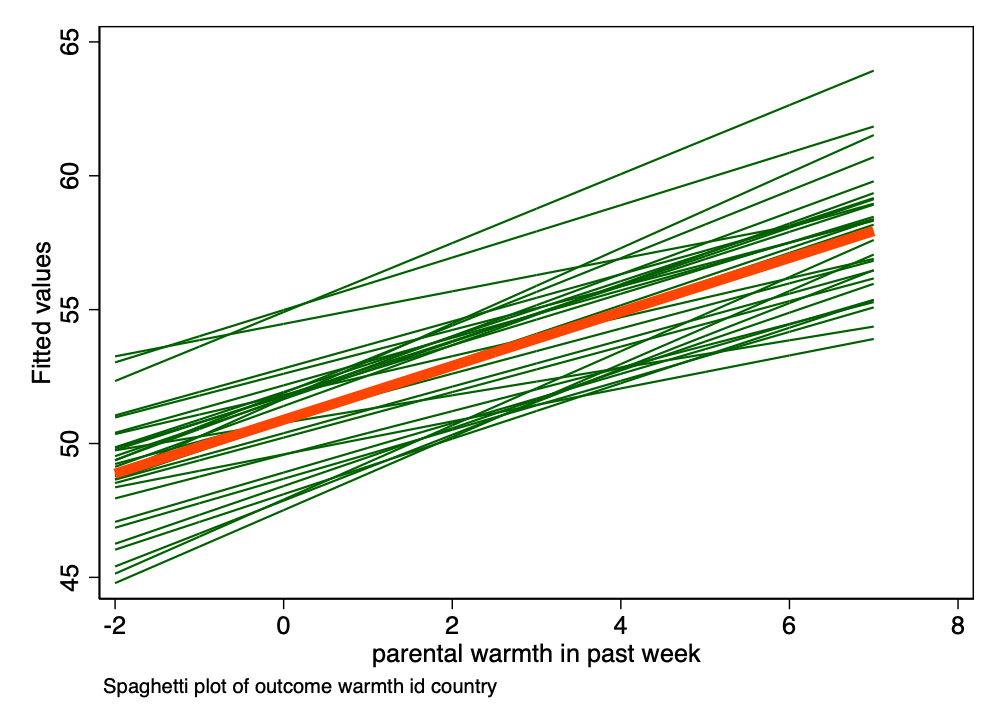
\includegraphics[width=0.5\linewidth,height=\textheight,keepaspectratio]{spagplot1.png}

}

\caption{Spaghetti Plot of Outcome by Warmth by Country}

\end{figure}%

\subsection{Unconditional Model}\label{unconditional-model}

\subsubsection{Model}\label{model}

\begin{Shaded}
\begin{Highlighting}[]

\NormalTok{mixed outcome || country: }\CommentTok{// unconditional model}
\end{Highlighting}
\end{Shaded}

\begin{verbatim}
Performing EM optimization ...

Performing gradient-based optimization: 
Iteration 0:  Log likelihood = -9802.8371  
Iteration 1:  Log likelihood = -9802.8371  

Computing standard errors ...

Mixed-effects ML regression                           Number of obs    = 3,000
Group variable: country                               Number of groups =    30
                                                      Obs per group:
                                                                   min =   100
                                                                   avg = 100.0
                                                                   max =   100
                                                      Wald chi2(0)     =     .
Log likelihood = -9802.8371                           Prob > chi2      =     .

------------------------------------------------------------------------------
     outcome | Coefficient  Std. err.      z    P>|z|     [95% conf. interval]
-------------+----------------------------------------------------------------
       _cons |   52.43327   .3451217   151.93   0.000     51.75685     53.1097
------------------------------------------------------------------------------

------------------------------------------------------------------------------
  Random-effects parameters  |   Estimate   Std. err.     [95% conf. interval]
-----------------------------+------------------------------------------------
country: Identity            |
                  var(_cons) |   3.178658   .9226737      1.799552    5.614658
-----------------------------+------------------------------------------------
               var(Residual) |   39.46106   1.024013      37.50421       41.52
------------------------------------------------------------------------------
LR test vs. linear model: chibar2(01) = 166.31        Prob >= chibar2 = 0.0000
\end{verbatim}

\subsubsection{ICC}\label{icc}

\begin{Shaded}
\begin{Highlighting}[]

\KeywordTok{estat}\NormalTok{ icc}
\end{Highlighting}
\end{Shaded}

\begin{verbatim}
Intraclass correlation

------------------------------------------------------------------------------
                       Level |        ICC   Std. err.     [95% conf. interval]
-----------------------------+------------------------------------------------
                     country |   .0745469   .0201254      .0434963    .1248696
------------------------------------------------------------------------------
\end{verbatim}

\subsection{Conditional Model}\label{conditional-model}

\begin{Shaded}
\begin{Highlighting}[]

\NormalTok{mixed outcome warmth physical\_punishment }\KeywordTok{identity}\NormalTok{ i.intervention HDI || country: warmth }\CommentTok{// multilevel model}

\KeywordTok{est} \KeywordTok{store}\NormalTok{ crosssectional }\CommentTok{// store estimates}
\end{Highlighting}
\end{Shaded}

\begin{verbatim}
Performing EM optimization ...

Performing gradient-based optimization: 
Iteration 0:  Log likelihood = -9626.6279  
Iteration 1:  Log likelihood =  -9626.607  
Iteration 2:  Log likelihood =  -9626.607  

Computing standard errors ...

Mixed-effects ML regression                          Number of obs    =  3,000
Group variable: country                              Number of groups =     30
                                                     Obs per group:
                                                                  min =    100
                                                                  avg =  100.0
                                                                  max =    100
                                                     Wald chi2(5)     = 334.14
Log likelihood =  -9626.607                          Prob > chi2      = 0.0000

-------------------------------------------------------------------------------------
            outcome | Coefficient  Std. err.      z    P>|z|     [95% conf. interval]
--------------------+----------------------------------------------------------------
             warmth |   .8345368   .0637213    13.10   0.000     .7096453    .9594282
physical_punishment |  -.9916657   .0797906   -12.43   0.000    -1.148052   -.8352791
           identity |  -.3004767   .2170295    -1.38   0.166    -.7258466    .1248933
     1.intervention |   .6396427   .2174519     2.94   0.003     .2134448    1.065841
                HDI |   -.003228   .0199257    -0.16   0.871    -.0422817    .0358256
              _cons |   51.99991   1.371257    37.92   0.000      49.3123    54.68753
-------------------------------------------------------------------------------------

------------------------------------------------------------------------------
  Random-effects parameters  |   Estimate   Std. err.     [95% conf. interval]
-----------------------------+------------------------------------------------
country: Independent         |
                 var(warmth) |   .0227504   .0257784      .0024689    .2096436
                  var(_cons) |   2.963975   .9737647      1.556777    5.643163
-----------------------------+------------------------------------------------
               var(Residual) |   34.97499   .9097109      33.23668    36.80422
------------------------------------------------------------------------------
LR test vs. linear model: chi2(2) = 205.74                Prob > chi2 = 0.0000

Note: LR test is conservative and provided only for reference.
\end{verbatim}

\section{Longitudinal Model}\label{longitudinal-model}

\subsection{Get Data}\label{get-data-1}

\begin{Shaded}
\begin{Highlighting}[]

\KeywordTok{use} \StringTok{"simulated\_multilevel\_longitudinal\_data.dta"}\NormalTok{, }\KeywordTok{clear}
\end{Highlighting}
\end{Shaded}

\subsection{The Equation}\label{the-equation-1}

\[\text{outcome}_{ij} = \beta_0 + \beta_1 \text{parental warmth} + \beta_2 \text{physical punishment} + \beta_3 \text{time} + \]

\[\beta_4 \text{identity}_2 + \beta_5 \text{intervention} + \beta_5 HDI +\]

\[u_{0j} + u_{1j} \times \text{parental warmth} + \]

\[v_{0i} + v_{1i} \times t + e_{ij} \]

\subsection{Descriptive Statistics}\label{descriptive-statistics-1}

\begin{Shaded}
\begin{Highlighting}[]

\KeywordTok{summarize} \CommentTok{// descriptive statistics}
\end{Highlighting}
\end{Shaded}

\begin{verbatim}
    Variable |        Obs        Mean    Std. dev.       Min        Max
-------------+---------------------------------------------------------
     country |      9,000        15.5    8.655922          1         30
         HDI |      9,000    64.76667     17.2437         33         87
      family |      9,000        50.5    28.86767          1        100
          id |          0
    identity |      9,000    .4976667    .5000223          0          1
-------------+---------------------------------------------------------
intervention |      9,000    .4843333    .4997823          0          1
           t |      9,000           2    .8165419          1          3
physical_p~t |      9,000    2.485333    1.373639          0          5
      warmth |      9,000    3.514222      1.8839          0          7
     outcome |      9,000    53.37768    6.572285   29.60798   79.02199
\end{verbatim}

\subsection{Alternate Plot}\label{alternate-plot}

\begin{Shaded}
\begin{Highlighting}[]
\KeywordTok{encode}\NormalTok{ id, }\KeywordTok{generate}\NormalTok{(idNUMERIC) }\CommentTok{// numeric version of id}
    
\NormalTok{* spagplot outcome t }\KeywordTok{if}\NormalTok{ idNUMERIC \textless{}= 10, id(idNUMERIC) }\DecValTok{scheme}\NormalTok{(stcolor)}
    
\KeywordTok{twoway}\NormalTok{ (}\KeywordTok{lfit}\NormalTok{ outcome t) (}\KeywordTok{scatter}\NormalTok{ outcome t) }\KeywordTok{if}\NormalTok{ idNUMERIC \textless{}= 10, }\KeywordTok{by}\NormalTok{(idNUMERIC) }\DecValTok{scheme}\NormalTok{(stcolor)}

\KeywordTok{graph} \KeywordTok{export}\NormalTok{ spagplot2.png, }\KeywordTok{width}\NormalTok{(1000) }\KeywordTok{replace}
\end{Highlighting}
\end{Shaded}

\begin{figure}[H]

{\centering 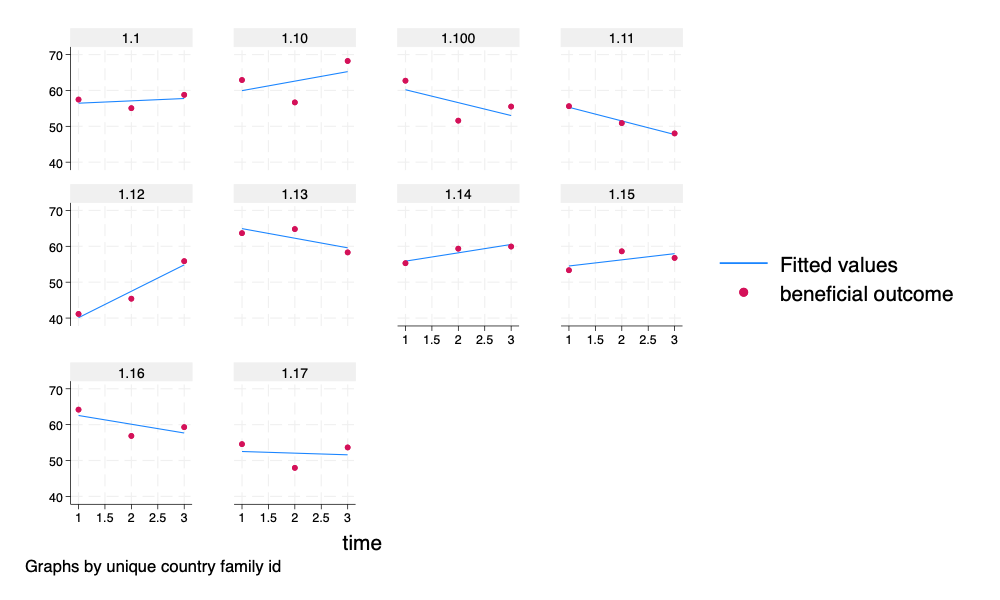
\includegraphics[width=0.5\linewidth,height=\textheight,keepaspectratio]{spagplot2.png}

}

\caption{Alternate Plot of Outcome by Time by Individual; First 10
Observations}

\end{figure}%

\subsection{Unconditional Model}\label{unconditional-model-1}

\subsubsection{Model}\label{model-1}

\begin{Shaded}
\begin{Highlighting}[]
\NormalTok{mixed outcome || country: || id: }\CommentTok{// unconditional model}
\end{Highlighting}
\end{Shaded}

\subsubsection{ICC}\label{icc-1}

\begin{Shaded}
\begin{Highlighting}[]

\KeywordTok{estat}\NormalTok{ icc}
\end{Highlighting}
\end{Shaded}

\begin{verbatim}
Intraclass correlation

------------------------------------------------------------------------------
                       Level |        ICC   Std. err.     [95% conf. interval]
-----------------------------+------------------------------------------------
                     country |   .0748336   .0190847      .0450028    .1219141
                  id|country |   .3462837   .0171461      .3134867    .3806097
------------------------------------------------------------------------------
\end{verbatim}

\subsection{Conditional Model}\label{conditional-model-1}

\begin{Shaded}
\begin{Highlighting}[]

\NormalTok{mixed outcome t warmth physical\_punishment i.}\KeywordTok{identity}\NormalTok{ i.intervention HDI || country: warmth || id: t }\CommentTok{// multilevel model}

\KeywordTok{est} \KeywordTok{store}\NormalTok{ longitudinal }\CommentTok{// store estimates}
\end{Highlighting}
\end{Shaded}

\begin{verbatim}
Performing EM optimization ...

Performing gradient-based optimization: 
Iteration 0:  Log likelihood =  -28523.49  
Iteration 1:  Log likelihood = -28499.987  
Iteration 2:  Log likelihood = -28499.739  
Iteration 3:  Log likelihood = -28499.604  
Iteration 4:  Log likelihood = -28499.603  

Computing standard errors ...

Mixed-effects ML regression                            Number of obs =   9,000

        Grouping information
        -------------------------------------------------------------
                        |     No. of       Observations per group
         Group variable |     groups    Minimum    Average    Maximum
        ----------------+--------------------------------------------
                country |         30        300      300.0        300
                     id |      3,000          3        3.0          3
        -------------------------------------------------------------

                                                       Wald chi2(6)  = 1096.15
Log likelihood = -28499.603                            Prob > chi2   =  0.0000

-------------------------------------------------------------------------------------
            outcome | Coefficient  Std. err.      z    P>|z|     [95% conf. interval]
--------------------+----------------------------------------------------------------
                  t |    .943864   .0658716    14.33   0.000      .814758     1.07297
             warmth |   .9134959   .0423732    21.56   0.000      .830446    .9965459
physical_punishment |  -1.007897   .0497622   -20.25   0.000    -1.105429   -.9103647
         1.identity |  -.1276926   .1515835    -0.84   0.400    -.4247908    .1694057
     1.intervention |   .8589966   .1519095     5.65   0.000     .5612596    1.156734
                HDI |  -.0005657   .0196437    -0.03   0.977    -.0390666    .0379352
              _cons |   50.46724   1.338318    37.71   0.000     47.84418    53.09029
-------------------------------------------------------------------------------------

------------------------------------------------------------------------------
  Random-effects parameters  |   Estimate   Std. err.     [95% conf. interval]
-----------------------------+------------------------------------------------
country: Independent         |
                 var(warmth) |   .0107586   .0127845      .0010478    .1104703
                  var(_cons) |   3.167085   .9146761      1.798154    5.578181
-----------------------------+------------------------------------------------
id: Independent              |
                      var(t) |   3.58e-09   7.06e-07      3.5e-177    3.7e+159
                  var(_cons) |   8.387275   .4724188      7.510631    9.366242
-----------------------------+------------------------------------------------
               var(Residual) |   26.02733   .4753701      25.11211    26.97592
------------------------------------------------------------------------------
LR test vs. linear model: chi2(4) = 1247.03               Prob > chi2 = 0.0000

Note: LR test is conservative and provided only for reference.
\end{verbatim}

\section{Nice Table of Results}\label{nice-table-of-results}

\begin{Shaded}
\begin{Highlighting}[]

\NormalTok{etable, }\KeywordTok{estimates}\NormalTok{(crosssectional longitudinal) }\CommentTok{///}
\NormalTok{showstars showstarsnote }\CommentTok{/// show stars and note}
\NormalTok{column(estimate) }\CommentTok{// column is modelname}
\end{Highlighting}
\end{Shaded}

\begin{verbatim}
                                     crosssectional longitudinal
----------------------------------------------------------------
parental warmth in past week             0.835 **      0.913 ** 
                                       (0.064)       (0.042)    
physical punishment in past week        -0.992 **     -1.008 ** 
                                       (0.080)       (0.050)    
hypothetical identity group variable    -0.300                  
                                       (0.217)                  
recieved intervention                                           
  1                                      0.640 **      0.859 ** 
                                       (0.217)       (0.152)    
Human Development Index                 -0.003        -0.001    
                                       (0.020)       (0.020)    
time                                                   0.944 ** 
                                                     (0.066)    
hypothetical identity group variable                            
  1                                                   -0.128    
                                                     (0.152)    
Intercept                               52.000 **     50.467 ** 
                                       (1.371)       (1.338)    
var(warmth)                              0.023         0.011    
                                       (0.026)       (0.013)    
var(_cons)                               2.964         3.167    
                                       (0.974)       (0.915)    
var(e)                                  34.975        26.027    
                                       (0.910)       (0.475)    
var(_cons)                                             8.387    
                                                     (0.472)    
var(t)                                                 0.000    
                                                     (0.000)    
Number of observations                    3000          9000    
----------------------------------------------------------------
** p<.01, * p<.05
\end{verbatim}

\section{QUESTIONS???}\label{majorsection}

\bookmarksetup{startatroot}

\chapter{Cross-Classified Models}\label{cross-classified-models}

\section{Introduction}\label{introduction-1}

A two level multilevel model imagines that \emph{Level 1} units are
nested in \emph{Level 2} units. A three level multilevel model imagines
that \emph{Level 1} units are nested in \emph{Level 2} units, which are
in turn nested in \emph{Level 3}.

A cross-classified model imagines that the nesting is not hierarchical,
but rather that there are two sets of clusters or nestings in which
individuals may be nested.

\section{Get Data}\label{get-data-2}

\begin{Shaded}
\begin{Highlighting}[]

\KeywordTok{use} \StringTok{"simulated\_multilevel\_longitudinal\_data.dta"}\NormalTok{, }\KeywordTok{clear}
\end{Highlighting}
\end{Shaded}

\section{Cross Classified Model}\label{cross-classified-model}

We can treat these random effects as being \emph{cross classified}.

This might be useful if we had data where individuals lived in different
countries at different times.

However, because \texttt{id} is in fact nested inside \texttt{country},
in this case, estimating the random effects as cross classified will be
more time consuming, but will give us equivalent results to a three
level model.

\subsection{Standard (Less Computationally Efficient)
Syntax}\label{standard-less-computationally-efficient-syntax}

The below syntax will take a very long time to run with the full sample,
and thus we have commented it out.

\begin{Shaded}
\begin{Highlighting}[]
    
\NormalTok{* mixed outcome t warmth physical\_punishment || }\DataTypeTok{\_all}\NormalTok{: R.country || }\DataTypeTok{\_all}\NormalTok{: R.id}
    
\NormalTok{* }\KeywordTok{est} \KeywordTok{store}\NormalTok{ crossed1}
\end{Highlighting}
\end{Shaded}

The documentation notes that we can use a \emph{much} more
computationally efficient version of the above command, which is what we
do in these notes. The user can verify that both versions of the command
will produce equivalent results.

In fact, at the end of handout we verify the similarity of both sets of
syntax using a random sample.

\subsection{Cross Classified With Computationally Efficient
Syntax}\label{cross-classified-with-computationally-efficient-syntax}

\begin{Shaded}
\begin{Highlighting}[]

\NormalTok{mixed outcome t warmth physical\_punishment || }\DataTypeTok{\_all}\NormalTok{: R.country || id:}
    
\KeywordTok{est} \KeywordTok{store}\NormalTok{ crossed2 }\CommentTok{// store crossed effects result}
\end{Highlighting}
\end{Shaded}

\begin{verbatim}
Performing EM optimization ...

Performing gradient-based optimization: 
Iteration 0:  Log likelihood = -28516.314  
Iteration 1:  Log likelihood = -28516.277  
Iteration 2:  Log likelihood = -28516.277  

Computing standard errors ...

Mixed-effects ML regression                            Number of obs =   9,000

        Grouping information
        -------------------------------------------------------------
                        |     No. of       Observations per group
         Group variable |     groups    Minimum    Average    Maximum
        ----------------+--------------------------------------------
                   _all |          1      9,000    9,000.0      9,000
                     id |      3,000          3        3.0          3
        -------------------------------------------------------------

                                                       Wald chi2(3)  = 1168.69
Log likelihood = -28516.277                            Prob > chi2   =  0.0000

-------------------------------------------------------------------------------------
            outcome | Coefficient  Std. err.      z    P>|z|     [95% conf. interval]
--------------------+----------------------------------------------------------------
                  t |   .9434605    .065866    14.32   0.000     .8143654    1.072556
             warmth |   .9053924   .0380439    23.80   0.000     .8308277    .9799572
physical_punishment |  -1.014385   .0499354   -20.31   0.000    -1.112257    -.916514
              _cons |    50.8301   .4123007   123.28   0.000       50.022    51.63819
-------------------------------------------------------------------------------------

------------------------------------------------------------------------------
  Random-effects parameters  |   Estimate   Std. err.     [95% conf. interval]
-----------------------------+------------------------------------------------
_all: Identity               |
              var(R.country) |   3.429974    .930313      2.015668    5.836634
-----------------------------+------------------------------------------------
id: Identity                 |
                  var(_cons) |   8.608872   .4757699      7.725107     9.59374
-----------------------------+------------------------------------------------
               var(Residual) |   26.02862   .4752444      25.11363    26.97695
------------------------------------------------------------------------------
LR test vs. linear model: chi2(2) = 1260.84               Prob > chi2 = 0.0000

Note: LR test is conservative and provided only for reference.
\end{verbatim}

\section{Three Level Model}\label{three-level-model}

\begin{Shaded}
\begin{Highlighting}[]

\NormalTok{mixed outcome t warmth physical\_punishment || country: || id:  }\CommentTok{// 3 level w/ random intercepts only}
    
\KeywordTok{est} \KeywordTok{store}\NormalTok{ threelevel }\CommentTok{// store random intercept model}
\end{Highlighting}
\end{Shaded}

\begin{verbatim}
Performing EM optimization ...

Performing gradient-based optimization: 
Iteration 0:  Log likelihood = -28516.314  
Iteration 1:  Log likelihood = -28516.277  
Iteration 2:  Log likelihood = -28516.277  

Computing standard errors ...

Mixed-effects ML regression                            Number of obs =   9,000

        Grouping information
        -------------------------------------------------------------
                        |     No. of       Observations per group
         Group variable |     groups    Minimum    Average    Maximum
        ----------------+--------------------------------------------
                country |         30        300      300.0        300
                     id |      3,000          3        3.0          3
        -------------------------------------------------------------

                                                       Wald chi2(3)  = 1168.69
Log likelihood = -28516.277                            Prob > chi2   =  0.0000

-------------------------------------------------------------------------------------
            outcome | Coefficient  Std. err.      z    P>|z|     [95% conf. interval]
--------------------+----------------------------------------------------------------
                  t |   .9434605    .065866    14.32   0.000     .8143654    1.072556
             warmth |   .9053924   .0380439    23.80   0.000     .8308277    .9799572
physical_punishment |  -1.014385   .0499354   -20.31   0.000    -1.112257    -.916514
              _cons |    50.8301   .4123007   123.28   0.000       50.022    51.63819
-------------------------------------------------------------------------------------

------------------------------------------------------------------------------
  Random-effects parameters  |   Estimate   Std. err.     [95% conf. interval]
-----------------------------+------------------------------------------------
country: Identity            |
                  var(_cons) |   3.429974    .930313      2.015668    5.836634
-----------------------------+------------------------------------------------
id: Identity                 |
                  var(_cons) |   8.608872   .4757699      7.725107     9.59374
-----------------------------+------------------------------------------------
               var(Residual) |   26.02862   .4752444      25.11363    26.97695
------------------------------------------------------------------------------
LR test vs. linear model: chi2(2) = 1260.84               Prob > chi2 = 0.0000

Note: LR test is conservative and provided only for reference.
\end{verbatim}

\section{Nice Table of Results of Three Level and Cross Classified
Model}\label{nice-table-of-results-of-three-level-and-cross-classified-model}

\begin{Shaded}
\begin{Highlighting}[]

\NormalTok{etable, }\KeywordTok{estimates}\NormalTok{(threelevel crossed2), }\CommentTok{///}
\NormalTok{showstars showstarsnote }\CommentTok{/// show stars and note}
\NormalTok{column(estimate) }\CommentTok{// column is modelname}
\end{Highlighting}
\end{Shaded}

\begin{verbatim}
invalid 'showstars' 
r(198);

r(198);
\end{verbatim}

\section{Verification of Syntax Equivalence for Cross Classified
Model}\label{verification-of-syntax-equivalence-for-cross-classified-model}

\begin{Shaded}
\begin{Highlighting}[]

\KeywordTok{keep} \KeywordTok{if} \KeywordTok{family}\NormalTok{ \textless{}= 5 }\CommentTok{// random sample of families}
    
\KeywordTok{quietly}\NormalTok{ mixed outcome t warmth physical\_punishment || }\DataTypeTok{\_all}\NormalTok{: R.country || }\DataTypeTok{\_all}\NormalTok{: R.id}
    
\KeywordTok{est} \KeywordTok{store}\NormalTok{ crossed1A }\CommentTok{// less efficient syntax}
    
\KeywordTok{quietly}\NormalTok{ mixed outcome t warmth physical\_punishment || }\DataTypeTok{\_all}\NormalTok{: R.country || id:}
    
\KeywordTok{est} \KeywordTok{store}\NormalTok{ crossed2A }\CommentTok{// more efficient syntax}
    
\NormalTok{etable, }\KeywordTok{estimates}\NormalTok{(crossed1A crossed2A) }\CommentTok{///}
\NormalTok{showstars showstarsnote }\CommentTok{/// show stars and note}
\NormalTok{column(estimate) }\CommentTok{// column is modelname}
\end{Highlighting}
\end{Shaded}

\begin{verbatim}
(8,550 observations deleted)






------------------------------------------------------
                                  crossed1A  crossed2A
------------------------------------------------------
time                               0.745 **   0.745 **
                                 (0.281)    (0.281)   
parental warmth in past week       0.871 **   0.871 **
                                 (0.160)    (0.160)   
physical punishment in past week  -1.262 **  -1.262 **
                                 (0.206)    (0.206)   
Intercept                         51.755 **  51.755 **
                                 (1.009)    (1.009)   
var(R_country)                     2.245      2.245   
                                 (1.319)    (1.319)   
var(R_id)                          5.425              
                                 (1.843)              
var(e)                            23.638     23.638   
                                 (1.933)    (1.933)   
var(_cons)                                    5.425   
                                            (1.843)   
Number of observations               450        450   
------------------------------------------------------
** p<.01, * p<.05
\end{verbatim}

\section{QUESTIONS???}\label{questions}




\end{document}
